\section{Layered Medium}

\textbf{(a)}

The equations are linear and homogeneous in the wave amplitudes, so the
solution is only determined up to an arbitrary scaling. We therefore fix
\[
x_1 = 1.
\]
Then the scattering coefficient becomes
\[
S=\frac{y_1}{x_1}=y_1.
\]

The remaining unknown amplitudes are
\[
x_2,\ldots,x_n,\qquad
y_1,\ldots,y_n,
\]
giving \(2n-1\) unknowns. The equations
\[
x_{i+1}=t_i x_i+r_i y_{i+1},\qquad
y_i=r_i x_i+t_i y_{i+1},
\quad i=1,\ldots,n-1,
\]
together with the boundary condition
\[
y_n=x_n,
\]
provide exactly \(2n-1\) linear equations.

Collecting the unknowns into the vector
\[
z=
\begin{bmatrix}
x_2 & \cdots & x_n &
y_1 & \cdots & y_n
\end{bmatrix}^{\top},
\]
the equations can be written in the form
\[
Az=b.
\]
Solving this linear system yields all wave amplitudes, and the scattering
coefficient is then
\[
S=y_1.
\]

\textbf{(b)}

For \(n=20\), \(t_i=0.96\), and \(r_i=0.02\), the computed scattering
coefficient is
\[
    S=0.4981789631969839.
\]

\begin{figure}[H]
    \centering
    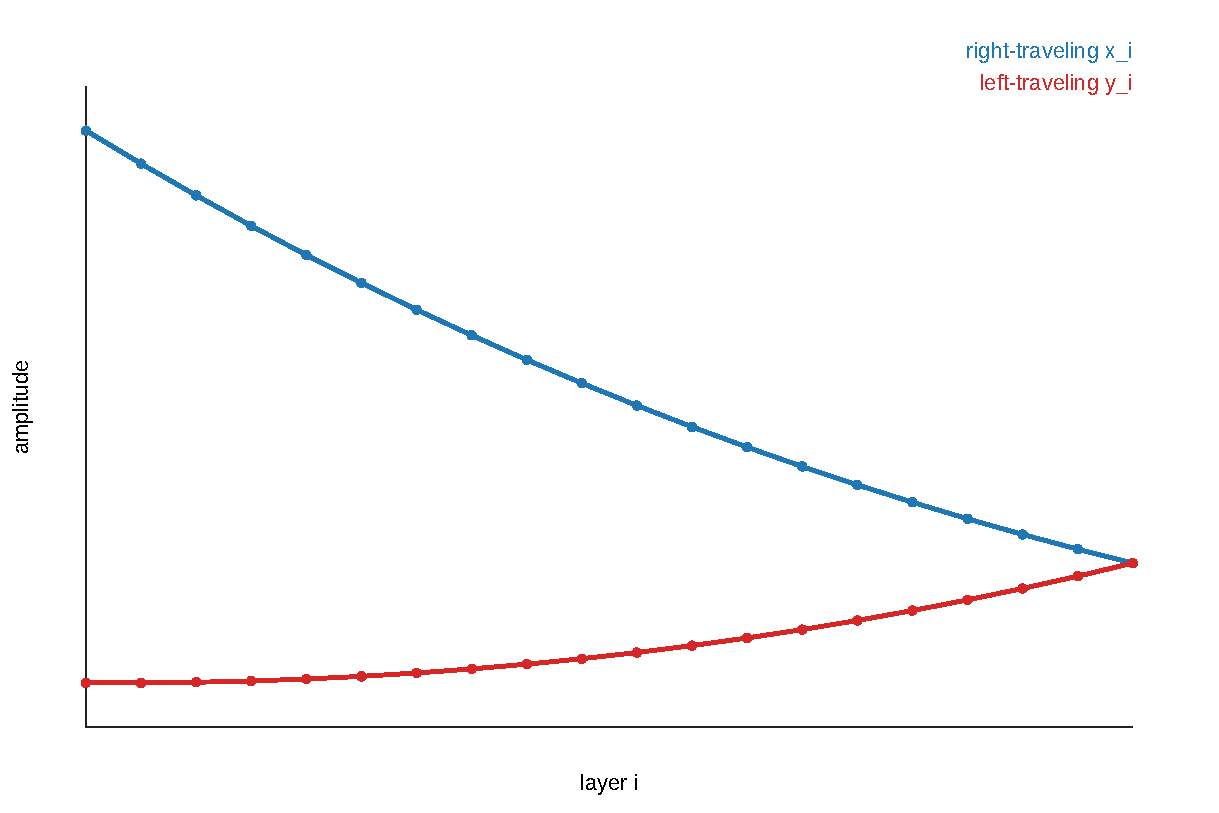
\includegraphics[width=0.82\textwidth]{img/p3_layered_medium.pdf}
    \caption{Right- and left-traveling wave amplitudes for the nominal medium.}
\end{figure}

\textbf{(c)}

For each candidate \(k\), set
\[
    t_k=0.02,\qquad r_k=0.96
\]
while keeping all other interfaces at the nominal values
\[
    t_i=0.96,\qquad r_i=0.02
\]
Then solve the same linear system as in part (a), producing a
coefficient \(S_k\). The most likely fault is the \(k\) minimizing
\[
    |S_k-S_{\mathrm{fault}}|
\]

% For \(S_{\mathrm{fault}}=0.70\), the closest match occurs at
% \[
%     k=9,
% \]
% where
% \[
%     S_9=0.7010126608436581.
% \]
% Thus interface \(9\) is most consistent with the measurement.

\begin{figure}[H]
    \centering
    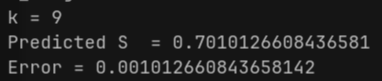
\includegraphics[width=0.65\textwidth]{img/3c.png}
\end{figure}

\textbf{Code}

\begin{lstlisting}
using LinearAlgebra

function solve_medium(t, r; x1=1.0)
    n = length(t) + 1
    nvars = 2n - 1
    A = zeros(nvars, nvars)
    b = zeros(nvars)

    idx_x(i) = i - 1
    idx_y(i) = (n - 1) + i

    row = 1
    for i in 1:(n - 1)
        A[row, idx_x(i + 1)] = 1.0
        if i == 1
            b[row] = t[i] * x1
        else
            A[row, idx_x(i)] = -t[i]
        end
        A[row, idx_y(i + 1)] = -r[i]
        row += 1

        A[row, idx_y(i)] = 1.0
        if i == 1
            b[row] = r[i] * x1
        else
            A[row, idx_x(i)] = -r[i]
        end
        A[row, idx_y(i + 1)] = -t[i]
        row += 1
    end

    A[row, idx_y(n)] = 1.0
    A[row, idx_x(n)] = -1.0

    z = A \ b
    x = [x1; z[1:(n - 1)]]
    y = z[n:end]
    return x, y, y[1] / x1
end

n = 20
t = fill(0.96, n - 1)
r = fill(0.02, n - 1)

x, y, S = solve_medium(t, r)
println("Nominal scattering coefficient S = ", S)

S_fault = 0.70
best_k = 0
best_S = 0.0
best_err = Inf

for k in 1:(n - 1)
    tk = copy(t)
    rk = copy(r)
    tk[k] = 0.02
    rk[k] = 0.96

    _, _, Sk = solve_medium(tk, rk)
    err = abs(Sk - S_fault)

    if err < best_err
        best_k = k
        best_S = Sk
        best_err = err
    end
end

println("k = ", best_k)
println("Predicted S = ", best_S)
println("Error = ", best_err)
\end{lstlisting}
